% =============================================================
% บทที่ 2 - ทฤษฎีและงานวิจัยที่เกี่ยวข้อง
% เนื้อหาแปลง/เรียบเรียงจาก Progress/Proposal Project1.docx ฉบับปรับปรุงล่าสุด (หัวข้อ 4)
% รวมหัวข้อ 4.3.4-4.3.5 (LLM-as-a-Judge, การประเมินผลการวางแผนการเดินทางด้วย LLM) ที่เพิ่มใหม่
% ฐานข้อมูล (PostgreSQL + pgvector) อัปเดตตาม proposal ฉบับใหม่ แทนที่ MongoDB+Chroma เดิมจาก Research Me
% =============================================================

% -----------------------------------------------------------
\section{ทฤษฎีที่เกี่ยวข้อง}
% -----------------------------------------------------------

ในยุคดิจิทัล การพัฒนาการท่องเที่ยวอัจฉริยะ (Smart Tourism) ได้กลายเป็นประเด็นที่ได้รับความสนใจจากนักวิจัยและผู้พัฒนาแพลตฟอร์มทั่วโลก อันเป็นผลมาจากพฤติกรรมนักท่องเที่ยวที่เปลี่ยนแปลงอย่างรวดเร็ว และความคาดหวังที่สูงขึ้นต่อข้อมูลที่ถูกต้อง การเข้าถึงบริการที่สะดวก รวมถึงประสบการณ์การท่องเที่ยวที่สามารถตอบสนองความต้องการเฉพาะบุคคล \parencite{sousa2024} ความท้าทายที่สำคัญจึงอยู่ที่การสร้างระบบที่สามารถนำเสนอข้อมูลแบบเรียลไทม์ ให้คำแนะนำที่แม่นยำ และสามารถปรับตามบริบทของผู้ใช้ได้อย่างมีประสิทธิภาพ

สำหรับจังหวัดขอนแก่น ซึ่งนับเป็นศูนย์กลางด้านการท่องเที่ยวของภาคตะวันออกเฉียงเหนือ ยังคงเผชิญกับปัญหาการกระจัดกระจายของข้อมูลการท่องเที่ยว แหล่งข้อมูลที่มีอยู่ในปัจจุบันมิได้ถูกรวบรวมอย่างเป็นระบบ ทำให้นักท่องเที่ยวที่ต้องการค้นหาแหล่งท่องเที่ยว ร้านอาหาร ที่พัก หรือกิจกรรมต่าง ๆ ต้องประสบความยากลำบากในการเข้าถึง อีกทั้งยังขาดเครื่องมือที่ช่วยในการวางแผนการเดินทางหรือแนะนำเส้นทางที่สอดคล้องกับความสนใจและงบประมาณของผู้ใช้ ส่งผลให้ประสบการณ์การท่องเที่ยวของจังหวัดขอนแก่นยังไม่สามารถสะท้อนศักยภาพที่มีอยู่ได้อย่างเต็มที่

เพื่อแก้ไขปัญหาดังกล่าว จึงได้มีการพัฒนาโครงงาน ``Dino: The central web application for tourism in Khon Kaen'' โดยมีเป้าหมายในการสร้างแพลตฟอร์มศูนย์กลางที่สามารถรวบรวมและจัดการข้อมูลด้านการท่องเที่ยวได้อย่างครบวงจร พร้อมทั้งบูรณาการเทคโนโลยีปัญญาประดิษฐ์ (Artificial Intelligence: AI) โดยเฉพาะโมเดลภาษาขนาดใหญ่ (LLMs) ร่วมกับสถาปัตยกรรม RAG เพื่อสนับสนุนการดำเนินงานใน 3 องค์ประกอบหลัก ได้แก่ ระบบฐานความรู้และการสืบค้นข้อมูล (Knowledge Retrieval System) ระบบวางแผนการเดินทาง (Trip Planning System) และระบบ Chatbot (Chatbot System)

งานวิจัยที่เกี่ยวข้องได้ชี้ให้เห็นว่า การประยุกต์ใช้ AI โดยเฉพาะการผสาน RAG สามารถเพิ่มความแม่นยำในการแนะนำข้อมูลและสร้างระบบที่ปรับตามบริบทของผู้ใช้ได้อย่างยั่งยืน \parencite{banerjee2025} ขณะเดียวกัน งานวิจัยอีกด้านหนึ่งเน้นไปที่การพัฒนาระบบวางแผนการเดินทางแบบเรียลไทม์ซึ่งช่วยเพิ่มประสิทธิภาพในการสร้างประสบการณ์ที่เหมาะสมกับความสนใจและงบประมาณของผู้ใช้ \parencite{deshmukh2025}

ดังนั้น โครงงาน Dino จึงมิใช่เพียงการสร้างเครื่องมือดิจิทัลเพื่ออำนวยความสะดวกแก่นักท่องเที่ยวเท่านั้น หากแต่ยังเป็นการบูรณาการองค์ความรู้จากงานวิจัยและเทคโนโลยีสมัยใหม่ เพื่อต่อยอดสู่การพัฒนากลไกการจัดการท่องเที่ยวที่ชาญฉลาด เพิ่มศักยภาพในการแข่งขัน และยกระดับจังหวัดขอนแก่นสู่การเป็นเมืองท่องเที่ยวอัจฉริยะอย่างยั่งยืน

\subsection{แนวคิดการท่องเที่ยวอัจฉริยะ (Smart Tourism)}

Smart Tourism คือการใช้เทคโนโลยีในการสร้างระบบนิเวศท่องเที่ยวที่เชื่อมโยงข้อมูล บริการ และประสบการณ์ของผู้ใช้ งานของ \textcite{ma2025} แสดงให้เห็นว่า AI สามารถช่วยวิเคราะห์พฤติกรรมการเดินทางของผู้ใช้และปรับปรุงการจัดการจุดหมายปลายทางแบบเรียลไทม์ ในขณะที่งานของ \textcite{milton2023} ได้สรุปแนวโน้มความท้าทายและโอกาสของการใช้ AI ใน Smart Tourism เช่น ปัญหาความเป็นส่วนตัวและธรรมาภิบาลข้อมูล

\subsection{ปัญญาประดิษฐ์ (Artificial Intelligence) ในการท่องเที่ยว}

ปัญญาประดิษฐ์ (AI) มีบทบาทสำคัญอย่างยิ่งในการปฏิวัติประสบการณ์ท่องเที่ยวยุคใหม่ เพราะช่วยให้แพลตฟอร์มสามารถวิเคราะห์พฤติกรรมและความต้องการของผู้ใช้แบบเรียลไทม์ งานของ \textcite{sousa2024} ศึกษามุมมองของนักท่องเที่ยวที่มีต่อการนำ AI มาใช้ในอุตสาหกรรมท่องเที่ยวและการบริการ พบว่านักท่องเที่ยวคาดหวังให้ระบบ AI สามารถให้คำแนะนำที่ ``แม่นยำ'' และ ``เหมาะสมกับบริบท'' แต่ในขณะเดียวกันยังมีความกังวลเรื่อง ความถูกต้องของข้อมูล และ ความเป็นส่วนตัว

ในขณะที่งานของ \textcite{milton2023} วิเคราะห์เชิงลึกเกี่ยวกับโอกาสและความท้าทายในการนำ AI มาใช้ โดยชี้ให้เห็นว่า AI ช่วยเพิ่มศักยภาพในด้าน การวิเคราะห์ข้อมูลขนาดใหญ่ (Big Data), การทำ personalization, และ การสร้างโมเดลทำนายพฤติกรรมนักท่องเที่ยว แต่ยังมีปัญหาเชิงเทคนิค เช่น การจัดการข้อมูลที่ซับซ้อนและการบูรณาการหลายแหล่งข้อมูลเข้าด้วยกัน

\subsection{การจัดการจุดหมายปลายทางและการมีส่วนร่วมของนักท่องเที่ยว}

แนวคิดการจัดการจุดหมายปลายทาง (Destination Management) และการสร้างประสบการณ์ที่ดึงดูดนักท่องเที่ยวมีความสำคัญอย่างมากในยุคที่ผู้ใช้ต้องการ ข้อมูลแบบเฉพาะบุคคล งานวิจัยของ \textcite{ma2025} นำเสนอการใช้ AI เพื่อวิเคราะห์ พฤติกรรมการเดินทางของผู้ใช้ ผ่านเทคนิค heatmap analytics และ data visualization ซึ่งช่วยให้ผู้พัฒนาระบบเข้าใจลักษณะการใช้งานของผู้ใช้และสามารถปรับกลยุทธ์การนำเสนอข้อมูลให้ตรงตามความสนใจของแต่ละคน

\begin{figure}[H]
\centering
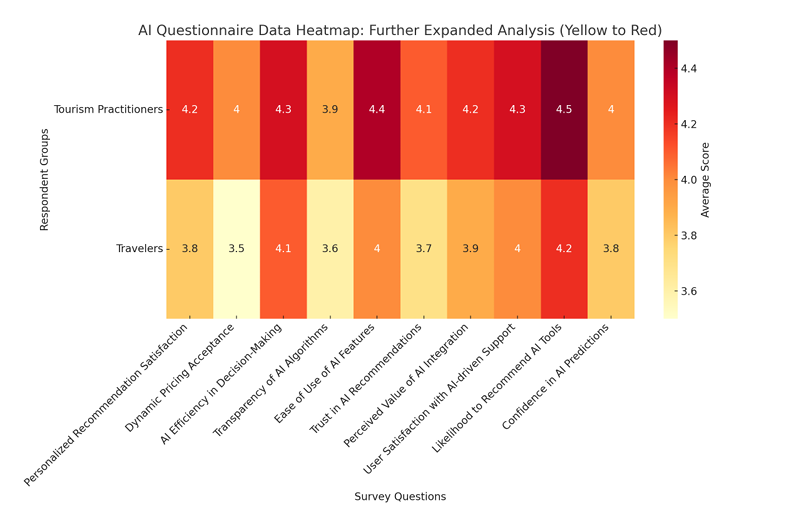
\includegraphics[width=0.7\textwidth]{images/image2.png}
\caption{แผนภาพ Heatmap แสดงข้อมูลจากแบบสอบถาม (Ma et al., 2025)}
\end{figure}

จากภาพข้างต้น แสดง Heatmap แสดงการประเมิน AI ของผู้ประกอบวิชาชีพและนักท่องเที่ยวใน 6 มิติ โดยใช้สีเหลือง--แดงแทนคะแนนต่ำ--สูง ผู้ประกอบวิชาชีพให้คะแนนสูงกว่าทุกมิติ โดยเฉพาะความง่ายในการใช้งานและประสิทธิภาพการตัดสินใจ ขณะที่นักท่องเที่ยวต่ำในด้านการยอมรับราคาไดนามิกและความโปร่งใสของอัลกอริทึม จึงควรปรับปรุงความโปร่งใสราคา กลยุทธ์ราคาไดนามิก และการควบคุมโดยผู้ใช้เพื่อเสริมสร้างความเชื่อมั่น

ผลการประเมินพบว่า ผู้ประกอบวิชาชีพให้คะแนนสูงกว่านักท่องเที่ยวในทุกมิติ โดยเฉพาะด้านความง่ายในการใช้งานคุณลักษณะ AI (4.4 เทียบกับ 4.0) และประสิทธิภาพการตัดสินใจที่เสริมด้วย AI (4.3 เทียบกับ 4.1) สะท้อนระดับความคุ้นเคยและความมั่นใจกับเทคโนโลยี AI ที่สูงกว่า ขณะที่นักท่องเที่ยวให้คะแนนต่ำอย่างมีนัยในมิติการยอมรับราคาแบบไดนามิก (3.5) และความโปร่งใสของอัลกอริทึม (3.6) บ่งชี้ถึงความไม่ไว้วางใจต่อระบบ AI ความกังวลต่อราคาที่ไม่โปร่งใส กลไกคำแนะนำที่เข้าใจยาก และความสงสัยต่อความเป็นธรรมของ AI ทั้งในด้านการกำหนดราคาและการตัดสินใจ ซึ่งอาจทำให้ผู้ใช้บางส่วนจ่ายแพงกว่า หรือได้รับคำแนะนำที่ด้อยกว่า

ในทางกลับกัน \textcite{banerjee2025} เสนอว่าการสร้าง ระบบแนะนำที่ยั่งยืน (sustainable recommendation) จะช่วยเพิ่ม การมีส่วนร่วม (engagement) ของนักท่องเที่ยวในระยะยาว โดยใช้ RAG ผสานข้อมูลเรียลไทม์จากหลายแหล่ง เพื่อสร้างการแนะนำที่แม่นยำและสอดคล้องกับบริบท

\subsection{ความยั่งยืน ความเสี่ยง และธรรมาภิบาลข้อมูล/อัลกอริทึม}

หนึ่งในประเด็นที่สำคัญสำหรับการพัฒนาแพลตฟอร์ม Smart Tourism คือการสร้างความสมดุลระหว่าง ประสบการณ์ผู้ใช้, ความยั่งยืน, และ การปกป้องข้อมูลส่วนบุคคล งานของ \textcite{banerjee2025} ชี้ให้เห็นว่าระบบแนะนำการท่องเที่ยวควรคำนึงถึง การใช้ทรัพยากรอย่างมีประสิทธิภาพ เพื่อลดผลกระทบทางสิ่งแวดล้อม เช่น การแนะนำเส้นทางที่ปล่อยคาร์บอนต่ำ

ในอีกมุมหนึ่ง งานของ \textcite{sousa2024} พบว่าผู้ใช้นักท่องเที่ยวให้ความสำคัญอย่างมากต่อ ความปลอดภัยของข้อมูล และความโปร่งใสของระบบ AI การละเลยประเด็นนี้อาจทำให้ผู้ใช้เกิดความไม่เชื่อมั่นและลดการมีส่วนร่วมในระยะยาว

\subsection{ทฤษฎีด้าน Chatbot}

การใช้ Chatbot ในอุตสาหกรรมการท่องเที่ยวได้พัฒนาอย่างก้าวกระโดดในช่วงไม่กี่ปีที่ผ่านมา โดยมีการบูรณาการ Artificial Intelligence Markup Language (AIML) และ Natural Language Processing (NLP) เพื่อสร้างระบบสนทนาที่สามารถตอบคำถามของผู้ใช้ได้แบบเรียลไทม์ \parencite{goizha2023} งานวิจัยพบว่า Chatbot สำหรับการท่องเที่ยวสามารถช่วยลดเวลาในการค้นหาข้อมูลได้เฉลี่ย 45\% และเพิ่มความพึงพอใจของนักท่องเที่ยวมากกว่า 70\% เมื่อเทียบกับการค้นหาข้อมูลแบบเดิม

\begin{figure}[H]
\centering
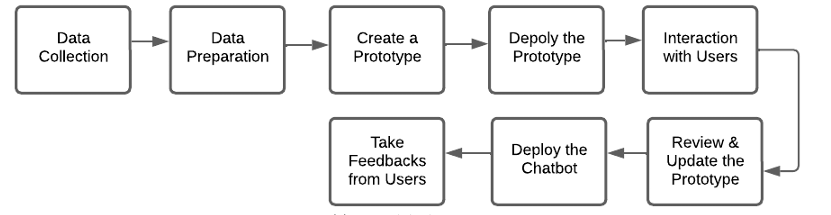
\includegraphics[width=0.7\textwidth]{images/image3.png}
\caption{แผนภาพ Model Flow (University College of Goizha et al., 2023)}
\end{figure}

จากภาพข้างต้น แสดงขั้นตอนและเทคนิคที่ใช้ในการเก็บรวบรวม วิเคราะห์ และตีความข้อมูลสำหรับการวิจัย โดยระเบียบวิธีประกอบด้วย 8 ขั้นตอน

\begin{enumerate}[label=(\arabic*)]
\item การเก็บรวบรวมข้อมูล: รวบรวมข้อมูลเกี่ยวกับเมือง Sulaimani ครอบคลุมโรงแรม ภัตตาคาร ศูนย์การค้า พิพิธภัณฑ์ และแหล่งท่องเที่ยวยอดนิยม
\item การเตรียมข้อมูล: จัดโครงสร้างข้อมูลให้อยู่ในรูปแบบชุดคำถาม--คำตอบ และบันทึกเป็นไฟล์ AIML
\item การสร้างต้นแบบ: สร้างแบบจำลองเริ่มต้นโดยใช้ไฟล์ AIML ที่จัดเตรียมไว้
\item การเผยแพร่ต้นแบบ: นำต้นแบบไปใช้งานบนเว็บไซต์ที่โฮสต์ภายในเครื่อง (local)
\item การโต้ตอบของผู้ใช้: ผู้ใช้ทำการโต้ตอบกับบอทที่ได้เผยแพร่
\item การปรับปรุงต้นแบบ: ทบทวนและแก้ไขต้นแบบตามข้อเสนอแนะและพฤติกรรมการใช้งานของผู้ใช้
\item การเผยแพร่โมเดลฉบับสมบูรณ์: เผยแพร่รุ่นสุดท้ายให้ผู้ใช้ใช้งานอีกครั้ง
\item ข้อเสนอแนะจากผู้ใช้: หลังการเผยแพร่และการใช้งานบอท รวบรวมข้อเสนอแนะเพื่อประเมินความพึงพอใจ ความสามารถในการใช้งาน (usability) และความมีส่วนร่วมของผู้ใช้
\end{enumerate}

ผลสำรวจของ \textcite{goizha2023} ยังชี้ว่า Chatbot แบบ AI ที่มีระบบเรียนรู้พฤติกรรมผู้ใช้ (Adaptive-Chatbot) สามารถแนะนำสถานที่ท่องเที่ยว ร้านอาหาร และกิจกรรมที่เหมาะสมได้อย่างแม่นยำถึง 82\% ทำให้ผู้ใช้รู้สึกว่าข้อมูลที่ได้รับมีความน่าเชื่อถือและเป็นประโยชน์มากกว่า Chatbot แบบ rule-based เดิม ๆ โดยมีนักท่องเที่ยวกว่า 64\% ระบุว่าพร้อมใช้ระบบนี้หากข้อมูลถูกปรับให้เหมาะสมกับตนเอง

นอกจากนี้ แนวโน้มในงานวิจัยล่าสุดได้ขยายขีดความสามารถของ Chatbot ให้รองรับการแปลภาษาอัตโนมัติ การแนะนำกิจกรรมตามฤดูกาล และการโต้ตอบแบบมัลติมีเดีย เช่น การส่งแผนที่ รูปภาพ และลิงก์ข้อมูลท่องเที่ยว \parencite{sousa2024} ซึ่งเป็นแนวคิดสำคัญสำหรับการพัฒนา Smart Tourism Applications ในอนาคต

\subsection{ระบบแนะนำการท่องเที่ยว (Recommendation Systems)}

การสร้างระบบแนะนำที่ตอบโจทย์ผู้ใช้เป็นหัวใจสำคัญสำหรับการท่องเที่ยวที่ตอบโจทย์ผู้ใช้แบบเฉพาะบุคคล (Personalized Experience) งานของ \textcite{banerjee2025} เสนอเทคนิค RAG ในการพัฒนาระบบแนะนำที่ใช้การเรียนรู้จากฐานข้อมูลจำนวนมหาศาลเพื่อสร้างข้อเสนอที่เหมาะสมที่สุดสำหรับผู้ใช้

ผลการทดลองของ \textcite{banerjee2025} พบว่าระบบ RAG-Based Tourism Recommender สามารถปรับปรุงความแม่นยำของคำแนะนำได้สูงถึง 91\% เมื่อเทียบกับวิธี Collaborative Filtering แบบดั้งเดิม ซึ่งช่วยลดเวลาในการค้นหาแผนการเดินทางจากเฉลี่ย 15 นาที เหลือเพียง 4 นาที นอกจากนี้ยังมีการประเมินความพึงพอใจของผู้ใช้ (User Satisfaction) พบว่าผู้ใช้กว่า 88\% พึงพอใจกับแผนการเดินทางที่ระบบแนะนำ

ในทำนองเดียวกัน งานของ \textcite{jyothi2025} ที่พัฒนา Travel Finder ซึ่งเป็นระบบแนะนำและจัดการทริปท่องเที่ยว พบว่าการใช้ Hybrid Recommendation (ผสม Content-Based + Collaborative Filtering) สามารถเพิ่มการมีส่วนร่วมของผู้ใช้มากกว่า 76\% และช่วยสร้างชุมชนของผู้เดินทางที่มีความสนใจคล้ายกัน ซึ่งเป็นแนวโน้มสำคัญของ Smart Tourism Ecosystem

\begin{figure}[H]
\centering
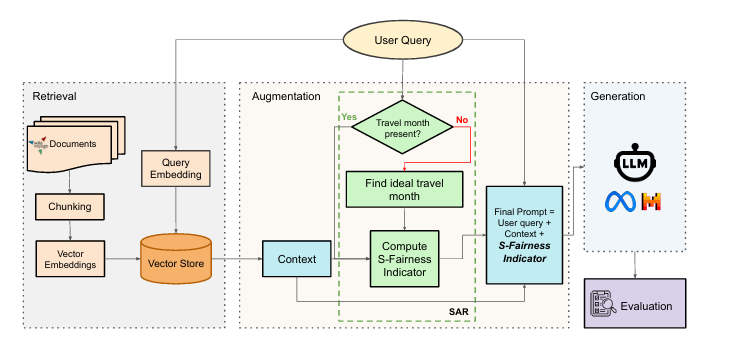
\includegraphics[width=0.7\textwidth]{images/image4.png}
\caption{แผนภาพ Pipeline ของระบบ RAG ที่ได้รับการปรับปรุงตามข้อเสนอโดยกรอบเส้นประสีเขียวแสดง ขั้นตอนการเสริมข้อมูลที่ปรับเปลี่ยน พร้อมการเพิ่มตัวชี้วัดด้านความยั่งยืน (Banerjee et al., 2025)}
\end{figure}

จากภาพข้างต้น อธิบายองค์ประกอบในการสร้างคำแนะนำการท่องเที่ยว

\textbf{Retrieval (การสืบค้นข้อมูล):} เริ่มจากการนำเอกสารข้อมูลแหล่งท่องเที่ยวมาแบ่งส่วน (Chunking) สร้างเวกเตอร์ฝังตัว (Vector Embeddings) และจัดเก็บในฐานข้อมูลเวกเตอร์ เมื่อผู้ใช้ป้อนคำถาม ระบบจะสร้างเวกเตอร์คำค้น (Query Embedding) เพื่อดึงข้อมูลหรือบริบท (Context) ที่มีความสอดคล้องและเกี่ยวข้องที่สุดออกมา

\textbf{Augmentation (การเสริมข้อมูล):} ระบบจะนำคำถามของผู้ใช้มารวมกับข้อมูลบริบทที่ดึงมาได้ เพื่อเสริมสร้างเป็น Prompt สุดท้ายที่มีความสมบูรณ์และมีข้อมูลอ้างอิงที่ถูกต้อง

\textbf{Generation (การสร้างคำตอบ):} ส่ง Prompt สุดท้ายที่ได้รับการเสริมข้อมูลแล้วไปให้โมเดลภาษาขนาดใหญ่ (LLM) ประมวลผลเพื่อสร้างคำตอบหรือแผนการเดินทางที่แม่นยำ พร้อมด้วยขั้นตอนการประเมินผล (Evaluation) ภายหลังการสร้างคำตอบ

\subsection{การสร้างแผนการเดินทาง (Trip Planning)}

การวางแผนการเดินทาง (Trip Planning) กำลังถูกประยุกต์ใช้ AI, Machine Learning และ Real-Time Data งานวิจัยของ \textcite{deshmukh2025} เสนอการพัฒนาระบบ AI-powered Trip Planner ที่ใช้ข้อมูลเรียลไทม์จากหลายแหล่ง เช่น สภาพอากาศ การจราจร ราคาที่พัก และความหนาแน่นของนักท่องเที่ยว เพื่อนำมาวิเคราะห์และสร้างแผนการเดินทางที่เหมาะสมที่สุด

ผลการทดลองพบว่า AI-powered Trip Planning สามารถปรับแผนการเดินทางให้เหมาะกับผู้ใช้แบบเรียลไทม์ และเพิ่มความแม่นยำในการแนะนำกิจกรรมได้สูงถึง 89\% ขณะที่ช่วยลดค่าใช้จ่ายเฉลี่ยต่อทริปได้มากกว่า 12\% เมื่อเทียบกับการวางแผนแบบ manual

\begin{figure}[H]
\centering
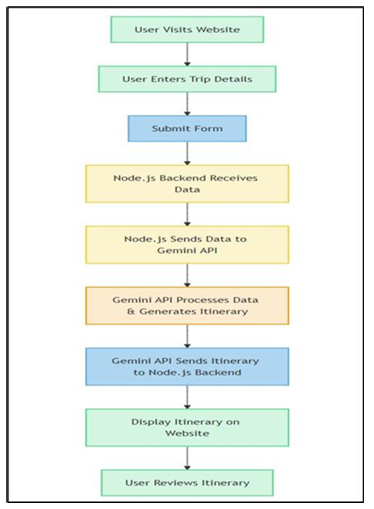
\includegraphics[width=0.7\textwidth]{images/image5.png}
\caption{แผนภาพสถาปัตยกรรมระบบ (Deshmukh et al., 2025)}
\end{figure}

จากภาพข้างต้น อธิบายองค์ประกอบและหน้าที่ของระบบวางแผนการเดินทางด้วย AI

\begin{enumerate}[label=(\arabic*)]
\item ผู้ใช้เข้าเว็บไซต์: กระบวนการเริ่มเมื่อผู้ใช้เปิดใช้งานเว็บแอปพลิเคชันผ่านอุปกรณ์ โดยแพลตฟอร์มจะแสดงอินเทอร์เฟซที่ใช้งานง่ายและสวยงามเพื่อแนะนำขั้นตอนการวางแผนทริป
\item ผู้ใช้กรอกรายละเอียดทริป: ผู้ใช้ป้อนข้อมูลที่เกี่ยวข้องกับการเดินทาง ได้แก่ จุดหมายปลายทาง วันที่เดินทาง ระยะเวลา งบประมาณ ความสนใจ/ความชอบ
\item ส่งแบบฟอร์ม: เมื่อกรอกข้อมูลครบถ้วน ผู้ใช้กดส่งแบบฟอร์ม เพื่อกระตุ้นให้มีการส่งคำขอไปยังระบบฝั่งเซิร์ฟเวอร์เพื่อประมวลผลต่อ
\item ระบบฝั่งเซิร์ฟเวอร์รับข้อมูล: จะรับข้อมูลแบบฟอร์ม พร้อมทั้งดูแลความปลอดภัย ตรวจสอบความถูกต้อง และจัดรูปแบบข้อมูลก่อนส่งต่อไปยังกระบวนการ AI
\item ระบบฝั่งเซิร์ฟเวอร์ส่งข้อมูลไปยังโมเดล AI: ระบบฝั่งเซิร์ฟเวอร์ส่งข้อมูลที่จัดโครงสร้างแล้วไปยังโมเดลภาษาขนาดใหญ่ ซึ่งทำหน้าที่ทำความเข้าใจเจตนา ความชอบของผู้ใช้ และปัจจัยเชิงบริบท เช่น สภาพอากาศปัจจุบันหรือแนวโน้มการท่องเที่ยว
\item โมเดล AI ประมวลผลและสร้างแผนการเดินทาง ด้วย NLP และอัลกอริทึม AI: ระบบจะตีความความต้องการของผู้ใช้และจัดทำแผนการเดินทางที่ปรับให้เหมาะสม โดยครอบคลุม กิจกรรมรายวัน คำแนะนำสถานที่ท่องเที่ยว ประสบการณ์ท้องถิ่นและร้านอาหาร วิธีการเดินทางและช่วงเวลา การผสานข้อมูลสภาพอากาศและคำแนะนำการเดินทางแบบเรียลไทม์
\item โมเดล AI ส่งแผนการเดินทางกลับมายังฝั่งเซิร์ฟเวอร์: เมื่อสร้างแผนเสร็จสิ้น ระบบจะส่งผลลัพธ์กลับมาที่ฝั่งเซิร์ฟเวอร์เพื่อจัดรูปแบบให้อยู่ในโครงสร้างที่เหมาะสมต่อการแสดงผลบนหน้าเว็บ
\item แสดงแผนการเดินทางบนเว็บไซต์: ส่วนติดต่อผู้ใช้จะแสดงแผนการเดินทางแบบไดนามิกด้วยโครงสร้างที่อ่านง่าย มีการแบ่งตามวัน แผนที่ ข้อเสนอแนะกิจกรรม และตัวเลือกการจองเพิ่มเติมตามความเหมาะสม
\end{enumerate}

ในอีกด้านหนึ่ง สำหรับการออกแบบสถาปัตยกรรมเพื่อรองรับการประมวลผลข้อมูลที่ซับซ้อน งานวิจัยของ \textcite{barua2024} ได้นำเสนอการใช้ สถาปัตยกรรมไมโครเซอร์วิส (Microservices Architecture) ซึ่งแบ่งการทำงานของระบบออกเป็นบริการย่อย ๆ (เช่น User Service, Itinerary Service และ Preference Matching Service) ที่ทำงานแยกจากกันแต่สามารถสื่อสารกันผ่าน API Gateway และ Message Broker สถาปัตยกรรมนี้ช่วยให้แพลตฟอร์มมีความยืดหยุ่น รองรับผู้ใช้งานจำนวนมากได้พร้อมกัน และสามารถประมวลผลแผนการเดินทางได้อย่างรวดเร็ว

\begin{figure}[H]
\centering
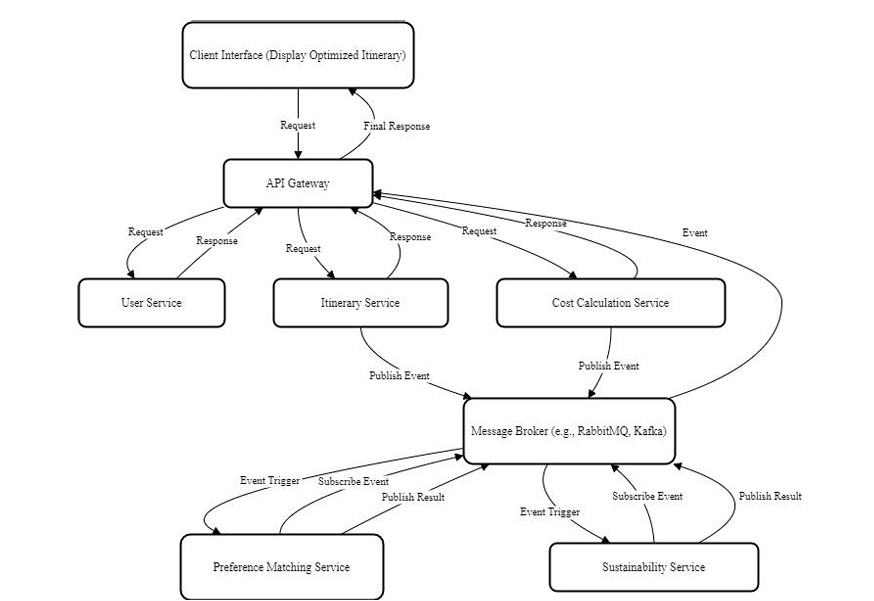
\includegraphics[width=0.7\textwidth]{images/image6.png}
\caption{แผนภาพการไหลของข้อมูลและกระบวนการประสานลำดับงาน (Barua \& Kaiser, 2024)}
\end{figure}

จากภาพข้างต้น อธิบายองค์ประกอบและหน้าที่ของกระบวนการไหลข้อมูลและการประสานงาน: คำขอจากไคลเอนต์ทั้งหมดถูกส่งไปยัง API Gateway ซึ่งทำหน้าที่เป็นจุดทางเข้าและกำหนดเส้นทางคำขอไปยังไมโครเซอร์วิสที่เกี่ยวข้อง (เช่น User Service, Itinerary Service, Cost Calculation Service) ผ่านทั้งการสื่อสารแบบซิงโครนัส (RESTful APIs) และแบบอะซิงโครนัสผ่านตัวกลางส่งข้อความ (Message Broker เช่น RabbitMQ หรือ Apache Kafka) สำหรับบริการที่ทำงานแบบขับเคลื่อนด้วยอีเวนต์ (เช่น Sustainability Service, Preference Matching Service) ก่อนที่ API Gateway จะรวบรวมผลลัพธ์และส่งต่อแผนการเดินทางที่ปรับให้เหมาะสมไปยังส่วนติดต่อผู้ใช้

อย่างไรก็ตาม ในส่วนของกลไกการคำนวณเพื่อสร้างแผนการเดินทางที่ต้องตอบสนองทั้งข้อจำกัดและความชอบส่วนบุคคลที่ซับซ้อน งานวิจัยล่าสุดของ \textcite{shao2025} ได้นำเสนอระบบ Personal Travel Solver (PTS) ซึ่งเปลี่ยนจากการใช้อัลกอริทึมค้นหาแบบดั้งเดิม (Heuristic Algorithms) มาเป็นการบูรณาการความสามารถของ โมเดลภาษาขนาดใหญ่ (LLMs) เข้ากับ ตัวแก้ปัญหาเชิงตัวเลข (Numerical Solvers) ระบบ PTS ใช้ LLM ในการตีความคำสั่งภาษาธรรมชาติของผู้ใช้และวิเคราะห์ประวัติรีวิวเพื่อสกัดเป็นคะแนนความพึงพอใจ (Preference Score) จากนั้นจะแปลงข้อมูลเหล่านี้ให้อยู่ในรูปแบบเชิงสัญลักษณ์ (Symbolic Representation) เพื่อส่งต่อให้ Mathematical Solver (เช่น SCIP Solver) ทำการคำนวณหาเส้นทางและตารางเวลาที่ดีที่สุดภายใต้ข้อจำกัด

\begin{figure}[H]
\centering
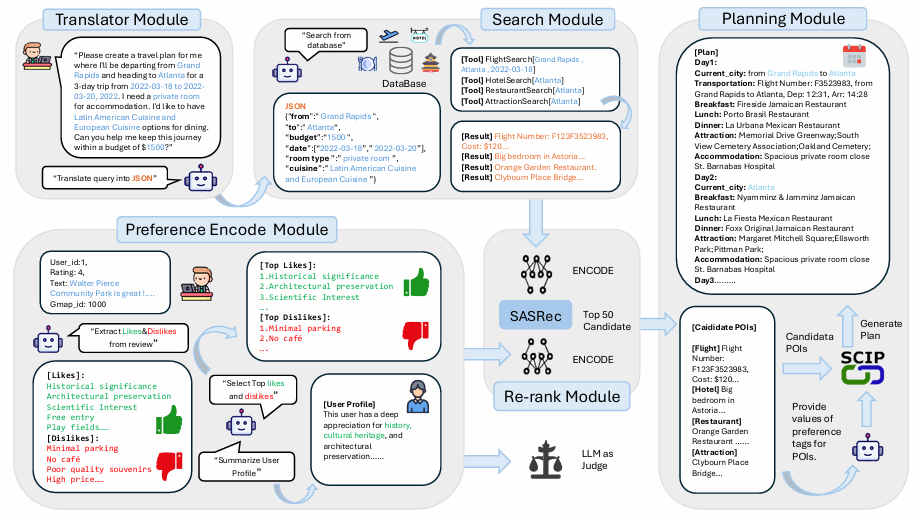
\includegraphics[width=0.7\textwidth]{images/image7.png}
\caption{แผนภาพสถาปัตยกรรมระบบ PTS (Personal Travel Solver Framework) (Shao et al., 2025)}
\end{figure}

จากภาพข้างต้น อธิบายองค์ประกอบและหน้าที่ของแผนภาพสถาปัตยกรรมระบบ PTS: โมดูลการแปลความหมาย (Translator Module) รับคำสั่งภาษาธรรมชาติและใช้ LLM แปลงเป็นรูปแบบเชิงสัญลักษณ์เพื่อสกัดข้อจำกัดที่ชัดเจน; โมดูลการค้นหา (Search Module) นำเงื่อนไขไปสืบค้นข้อมูลเบื้องต้นจากฐานข้อมูล; โมดูลเข้ารหัสความชอบ (Preference Encode Module) ใช้ LLM วิเคราะห์ประวัติการรีวิวเพื่อสกัดคะแนนความพึงพอใจ; โมดูลจัดอันดับใหม่ (Re-rank Module) จัดเรียงลำดับผลลัพธ์ตามคะแนนความพึงพอใจ; และโมดูลการวางแผน (Planning Module) ส่งข้อมูลที่คัดกรองแล้วเข้าสู่ตัวแก้ปัญหาทางคณิตศาสตร์เพื่อคำนวณและจัดตารางเวลาที่สมบูรณ์แบบ

% -----------------------------------------------------------
\section{งานวิจัยที่เกี่ยวข้อง}
% -----------------------------------------------------------

การศึกษางานวิจัยที่เกี่ยวข้องถือเป็นขั้นตอนสำคัญสำหรับการสร้างกรอบแนวคิดในการพัฒนา Dino: The central web application for tourism in Khon Kaen ซึ่งมุ่งพัฒนาแพลตฟอร์มศูนย์กลางเพื่อสนับสนุนการท่องเที่ยวในจังหวัดขอนแก่น โดยรวบรวมข้อมูลแหล่งท่องเที่ยว ร้านอาหาร ที่พัก กิจกรรม และบริการต่าง ๆ พร้อมระบบวางแผนการเดินทางที่ใช้ปัญญาประดิษฐ์ (AI) เพื่อช่วยสร้างประสบการณ์การท่องเที่ยวที่เหมาะสมกับความต้องการของผู้ใช้งาน

เพื่อตอบโจทย์นี้ มีการทบทวนงานวิจัย 11 ชิ้น ที่เกี่ยวข้องกับ AI, Smart Tourism, Recommendation Systems, Chatbots, Sustainable Tourism, Traveler Engagement, Microservices Architecture และการประเมินผลระบบวางแผนการเดินทางด้วย LLM ซึ่งช่วยให้เห็นแนวโน้มหลักในการออกแบบระบบท่องเที่ยวอัจฉริยะ รวมถึงช่องว่างขององค์ความรู้ (Research Gaps) และแนวทางการต่อยอด (Implications) ที่ Dino สามารถพัฒนาได้

\subsection{การใช้ AI เพื่อพัฒนาระบบแนะนำการท่องเที่ยวและ Trip Planning}

งานของ \textcite{banerjee2025} นำเสนอการใช้ RAG เพื่อพัฒนาระบบแนะนำการท่องเที่ยวแบบยั่งยืน โดยระบบจะดึงข้อมูลจากหลายแหล่ง เช่น บทความรีวิว สถิติการท่องเที่ยว และโซเชียลมีเดีย จากนั้นสร้างคำแนะนำที่เหมาะสมกับความสนใจเฉพาะบุคคลมากขึ้น ซึ่งช่วยปรับปรุงคุณภาพของคำแนะนำให้ตรงกับโปรไฟล์ของผู้ใช้งาน

ผลการศึกษานี้สอดคล้องกับงานของ \textcite{jyothi2025} ที่พัฒนา Travel Finder ซึ่งใช้ Collaborative Filtering และ Clustering Algorithms เพื่อสร้างกลุ่มนักท่องเที่ยวตามความสนใจและลักษณะการเดินทาง ผลการทดลองพบว่าระบบสามารถลดเวลาในการค้นหาแหล่งท่องเที่ยวลง 34\% และเพิ่มความพึงพอใจของผู้ใช้งานได้อย่างมีนัยสำคัญ ซึ่งสนับสนุนข้อค้นพบของ Banerjee et al. (2025) ว่าการใช้ AI เพื่อปรับคำแนะนำให้ตรงกับความต้องการส่วนบุคคล (Personalization) เป็นปัจจัยสำคัญต่อประสบการณ์ของนักท่องเที่ยว

อย่างไรก็ตาม ทั้งสองงานมีความแตกต่างกันในด้านแนวทาง Banerjee et al. (2025) มุ่งเน้นการสร้างระบบแนะนำเชิงข้อมูลเชิงลึก (Data-driven Recommendations) ผ่านการใช้โมเดลภาษาขนาดใหญ่ (LLMs) ขณะที่ Travel Finder ของ Jyothi et al. (2025) มุ่งเน้นการจับกลุ่มผู้ใช้ตามพฤติกรรมจริงเพื่อต่อยอดการแนะนำแบบ Social-based Recommendation ความแตกต่างนี้เปิดโอกาสให้ Dino สามารถผสมผสานข้อดีของทั้งสองวิธีเพื่อสร้างระบบที่ทั้ง แม่นยำ และ ยืดหยุ่น ในการแนะนำเส้นทางและกิจกรรมการท่องเที่ยว

\subsection{AI และ Chatbot เพื่อยกระดับประสบการณ์ผู้ใช้}

\textcite{goizha2023} พัฒนาระบบ Chatbot Tourist Guide โดยใช้ AIML เพื่อสร้างการสนทนาที่เป็นธรรมชาติกับนักท่องเที่ยว ระบบนี้สามารถตอบคำถามพื้นฐาน เช่น สถานที่ท่องเที่ยว ร้านอาหาร และข้อมูลตั๋วเข้าชม ผลการทดลองกับนักท่องเที่ยว 150 คน พบว่า 78\% ของผู้ใช้พึงพอใจกับความเร็วและความถูกต้องของคำตอบ นอกจากนี้ Chatbot ยังช่วยลดภาระงานของเจ้าหน้าที่ศูนย์บริการนักท่องเที่ยวลงถึง 40\%

ผลนี้สอดคล้องกับงานของ \textcite{deshmukh2025} ที่พัฒนาแพลตฟอร์ม AI-powered Personalized Itinerary Planning ซึ่งมี Chatbot ทำงานร่วมกับ Recommendation Engine เพื่อสร้างแผนการท่องเที่ยวอัตโนมัติ โดย Chatbot สามารถดึงข้อมูลแบบเรียลไทม์ เช่น สภาพอากาศ การจราจร และราคาที่พัก เพื่อปรับคำแนะนำให้สอดคล้องกับสถานการณ์ปัจจุบัน ผลการทดสอบกับกลุ่มนักท่องเที่ยว 300 คน พบว่า 85\% ของผู้ใช้ยืนยันว่าแผนการเดินทางที่ระบบสร้างให้มีความเหมาะสมและตรงตามความต้องการสูง

จากการสังเคราะห์ พบว่าทั้งสองงานสนับสนุนข้อสรุปสำคัญว่า Chatbot ไม่ได้เป็นเพียงเครื่องมืออำนวยความสะดวก แต่สามารถทำหน้าที่เป็น ตัวกลางในการวิเคราะห์ข้อมูลแบบเรียลไทม์ ซึ่งช่วยปรับแผนการท่องเที่ยวให้เหมาะสมมากขึ้น อย่างไรก็ตาม ความแตกต่างระหว่าง AIML-based Chatbot ของ \textcite{goizha2023} และระบบ AI-integrated Chatbot ของ \textcite{deshmukh2025} แสดงให้เห็นโอกาสในการพัฒนา Dino ให้รองรับ Natural Language Processing (NLP) ที่มีความฉลาดและยืดหยุ่นมากยิ่งขึ้น

\subsection{การจัดการข้อมูล การวิเคราะห์พฤติกรรม และการมีส่วนร่วมของนักท่องเที่ยว}

\textcite{ma2025} ศึกษาการใช้ AI เพื่อเพิ่มการมีส่วนร่วมของนักท่องเที่ยว (Traveler Engagement) และการจัดการจุดหมายปลายทาง (Destination Management) โดยใช้เทคนิค Heatmap Analytics และ Real-time Behavioral Tracking เพื่อระบุพื้นที่ที่นักท่องเที่ยวให้ความสนใจสูง ผลการทดลองแสดงให้เห็นว่าข้อมูลเชิงพฤติกรรมช่วยให้หน่วยงานท้องถิ่นปรับปรุงการจัดสรรทรัพยากรและออกแบบแผนการตลาดที่ตอบโจทย์ได้มากขึ้น

\begin{figure}[H]
\centering
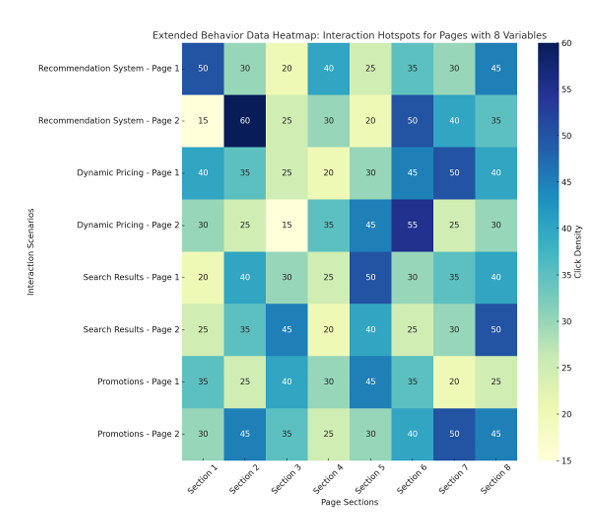
\includegraphics[width=0.7\textwidth]{images/image8.png}
\caption{แผนภาพ Heatmap แสดงข้อมูลเชิงพฤติกรรม (Ma et al., 2025)}
\end{figure}

การวิเคราะห์ Heatmap ของข้อมูลพฤติกรรมผู้ใช้จากสามแพลตฟอร์มท่องเที่ยวออนไลน์แสดงในภาพข้างต้น สื่อถึงการกระจาย ``ความเข้มข้นของการปฏิสัมพันธ์'' ของผู้ใช้ในส่วนต่าง ๆ ได้แก่ ระบบแนะนำ การกำหนดราคาแบบไดนามิก ผลการค้นหา และหน้าโปรโมชัน

ขณะเดียวกัน \textcite{sousa2024} ทำการสำรวจความคิดเห็นนักท่องเที่ยวจำนวน 500 คน เกี่ยวกับการใช้ AI ในการวางแผนการเดินทางและการเข้าถึงข้อมูล ผลการศึกษาพบว่า 72\% ของนักท่องเที่ยวเลือกใช้แพลตฟอร์มที่มี AI ในการแนะนำสถานที่ท่องเที่ยว และ 68\% ยืนยันว่าพวกเขามีแนวโน้มที่จะกลับมาใช้บริการซ้ำ หากระบบสามารถปรับคำแนะนำให้เหมาะกับพฤติกรรมการท่องเที่ยวส่วนบุคคล

การเปรียบเทียบสองงานนี้พบว่าทั้ง Ma et al. (2025) และ Sousa et al. (2024) ชี้ให้เห็นถึงความสำคัญของ Data-driven Personalization และ Traveler Engagement แต่ต่างกันที่ Ma et al. (2025) มุ่งเน้นการวิเคราะห์เชิงเทคนิคเพื่อช่วยองค์กรปรับปรุงโครงสร้างการจัดการ ขณะที่ Sousa et al. (2024) มุ่งสำรวจพฤติกรรมและความต้องการของผู้บริโภคโดยตรง ซึ่งแสดงให้เห็นว่าการพัฒนา Dino ควรผสมผสานข้อมูลทั้งสองฝั่งเข้าด้วยกันเพื่อให้เกิดแพลตฟอร์มที่ ตอบโจทย์ทั้งนักท่องเที่ยวและผู้กำหนดนโยบาย

\subsection{การประเมินผลด้วยโมเดลภาษาขนาดใหญ่ในฐานะผู้ประเมิน (LLM-as-a-Judge)}

งานวิจัยสำรวจเชิงลึกโดย \textcite{gu2025} ได้วิเคราะห์ขีดความสามารถและความน่าเชื่อถือของกรอบการทำงานแบบ LLM-as-a-Judge อย่างเป็นระบบ โดยระบุว่าโมเดลภาษาขนาดใหญ่มีความสามารถในการตีความภาษาธรรมชาติและจำลองกระบวนการตัดสินใจได้ใกล้เคียงกับมนุษย์ ส่งผลให้มีความยืดหยุ่นในการประเมินคำตอบเชิงคุณภาพที่มีลักษณะปลายเปิด (Open-ended Evaluation) ได้อย่างมีประสิทธิภาพ เหนือกว่าตัววัดผลเชิงสถิติแบบดั้งเดิม อีกทั้งยังช่วยลดต้นทุนและระยะเวลาในการทดสอบระบบลงอย่างมีนัยสำคัญ อย่างไรก็ตาม งานวิจัยดังกล่าวยังชี้ให้เห็นถึงข้อจำกัดและอคติแฝงของโมเดลภาษาในฐานะผู้ประเมิน เช่น อคติจากความยาวของคำตอบ (Verbosity Bias) อคติจากลำดับตัวเลือก (Position Bias) และความผันผวนของการให้คะแนน จึงเสนอกลไกเพิ่มความน่าเชื่อถือของการประเมินผ่านการกำหนดเกณฑ์การให้คะแนนที่ชัดเจน (Rubrics) การใช้คำตอบอ้างอิงประกอบการตัดสิน (Reference-based Evaluation) และการประเมินซ้ำเพื่อหาค่าเฉลี่ยสถิติ ซึ่งช่วยเพิ่มระดับความสอดคล้องระหว่างการประเมินของโมเดลและมนุษย์ (Human Alignment) ได้อย่างมีประสิทธิภาพ

\begin{figure}[H]
\centering
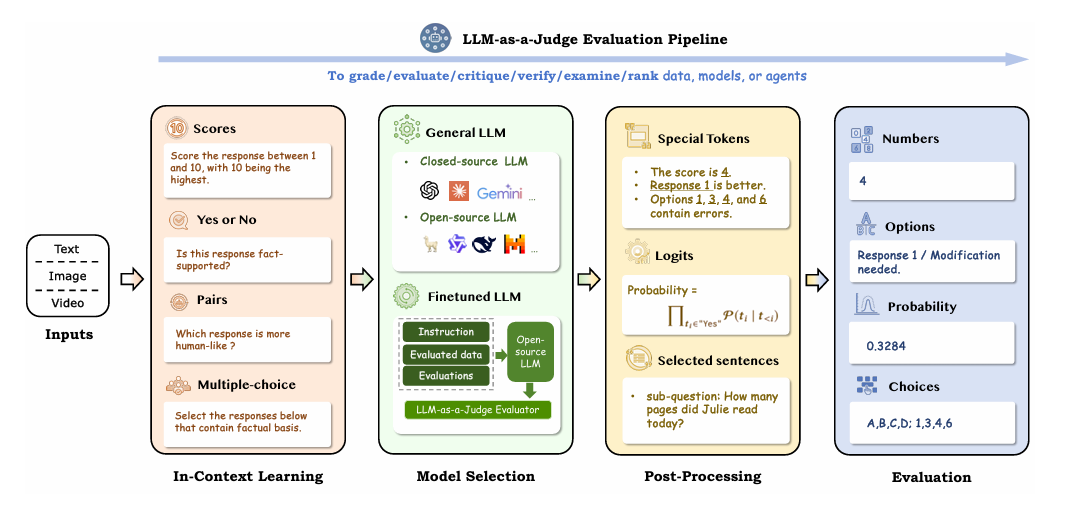
\includegraphics[width=0.7\textwidth]{images/image9.png}
\caption{สถาปัตยกรรมกระบวนการประเมินผลและการประมวลผลคำตอบของ LLM-as-a-Judge (Gu et al., 2025)}
\end{figure}

จากภาพข้างต้น แสดงกรอบแนวคิดกระบวนการประเมินแบบ LLM-as-a-Judge ซึ่งเริ่มต้นจากการรับโจทย์/คำสั่ง (Prompt/Query) และคำตอบที่ต้องการประเมิน (Candidate Response) ป้อนเข้าสู่โมเดลภาษาขนาดใหญ่ที่ทำหน้าที่เป็นผู้ประเมิน (Judge Model) โดยผ่านกลไกการกำหนดเกณฑ์ (Rubrics) และคำตอบอ้างอิง (Reference Answer) จากนั้นโมเดลจะสร้างกระบวนการวิเคราะห์เชิงตรรกะแบบ Chain-of-Thought (CoT) เพื่อให้เหตุผลรองรับ ก่อนส่งออกผลการประเมินในรูปแบบคะแนนเชิงปริมาณหรือการจัดอันดับคุณภาพ ซึ่งช่วยลดความผันผวนและเพิ่มความน่าเชื่อถือของการประเมินผลระบบตอบโต้

จากการวิเคราะห์งานวิจัยของ Gu et al. (2025) โครงงาน Dino จึงได้นำแนวคิด LLM-as-a-Judge มาประยุกต์ใช้ในส่วนการประเมินผลระบบตอบโต้และคำแนะนำสถานที่ท่องเที่ยว โดยตระหนักถึงทั้งจุดเด่นด้านความรวดเร็วและข้อควรระวังเรื่องอคติของโมเดล ระบบจึงออกแบบให้มีการกำหนดเกณฑ์การประเมินความถูกต้องของเนื้อหาเชิงประวัติศาสตร์และวัฒนธรรมของจังหวัดขอนแก่นอย่างรัดกุม ร่วมกับการใช้กลไก Chain-of-Thought เพื่อบังคับให้โมเดลผู้ประเมินแสดงเหตุผลประกอบก่อนสรุปคะแนน ส่งผลให้กระบวนการวัดผลของโครงงานมีความน่าเชื่อถือ โปร่งใส และรองรับการทดสอบในปริมาณมากได้อย่างมีประสิทธิภาพ

\subsection{การประเมินผลและวัดประสิทธิภาพการวางแผนการเดินทางด้วย LLM}

การประยุกต์ใช้โมเดลภาษาขนาดใหญ่ในระบบวางแผนการเดินทาง (Trip Planning) และระบบแนะนำสถานที่ท่องเที่ยว ได้รับความสนใจอย่างแพร่หลายในปัจจุบัน อย่างไรก็ตาม ความท้าทายสำคัญของโมเดลภาษาขนาดใหญ่คือการประมวลผลข้อจำกัดเชิงตรรกะที่ซับซ้อน การคำนวณตารางเวลาและงบประมาณผิดพลาด ตลอดจนการเกิดปัญหาการสร้างข้อมูลเท็จ ด้วยเหตุนี้ จึงเกิดแนวทางการพัฒนากรอบการประเมินเพื่อวัดประสิทธิภาพของระบบวางแผนการเดินทางด้วยปัญญาประดิษฐ์ในบริบทการใช้งานจริงอย่างเป็นระบบ

งานวิจัยของ \textcite{xie2024} ได้เสนอกรอบการประเมิน TravelPlanner ซึ่งเป็น Benchmark มาตรฐานสำหรับทดสอบขีดความสามารถของ AI Agents ในการวางแผนการเดินทางในโลกจริง งานวิจัยดังกล่าวเกิดขึ้นจากข้อจำกัดของการประเมินแบบดั้งเดิมที่มักวัดผลเฉพาะภารกิจการตอบคำถามสั้น ๆ ซึ่งไม่ครอบคลุมกระบวนการตัดสินใจหลายขั้นตอน (Complex Multi-step Tasks) โดยกำหนดให้ตัวแทนปัญญาประดิษฐ์ทำหน้าที่ดึงข้อมูลผ่านการเชื่อมต่อ API กับฐานข้อมูลจำลอง แล้วนำมาประเมินความถูกต้องของแผนการเดินทาง (Pass Rate) ใน 3 มิติหลัก ได้แก่ ข้อจำกัดเชิงสภาพแวดล้อม (Environment Constraints) เพื่อตรวจสอบว่าสถานที่ เที่ยวบิน หรือโรงแรม มีอยู่จริงในฐานข้อมูลโดยไม่เกิดการหลอนข้อมูล ข้อจำกัดเชิงสามัญสำนึก (Commonsense Constraints) เพื่อประเมินความสมเหตุสมผลของตารางเวลา และข้อจำกัดตามเงื่อนไขผู้ใช้ (Hard Constraints) เพื่อตรวจสอบความถูกต้องด้านงบประมาณและเงื่อนไขเฉพาะบุคคล

\begin{figure}[H]
\centering
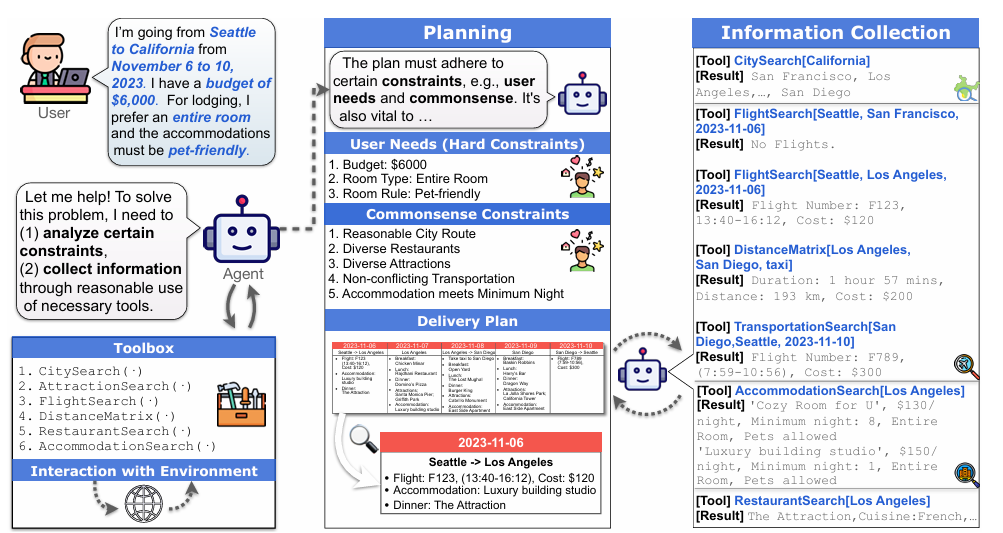
\includegraphics[width=0.7\textwidth]{images/image10.png}
\caption{กรอบแนวคิดการประเมินการวางแผนการเดินทาง (Xie et al., 2024)}
\end{figure}

ผลการทดลองของ Xie et al. (2024) พบว่าโมเดลภาษาขนาดใหญ่ระดับนำส่วนใหญ่มีอัตราการผ่านเกณฑ์ซับซ้อนสมบูรณ์ต่ำกว่าร้อยละ 10 เนื่องจากมักพบปัญหาการคำนวณงบประมาณสะสมผิดพลาดและการจัดตารางเวลาที่ขัดกับสามัญสำนึก

ขณะเดียวกัน \textcite{zheng2024} จาก Google DeepMind ได้เสนอแนวทางการประเมิน NATURAL PLAN เพื่อทดสอบขีดความสามารถเชิงตรรกะและการวางแผน (Natural Language Planning) ของโมเดลภาษาขนาดใหญ่เมื่อต้องรับคำสั่งภาษาธรรมชาติที่มีข้อจำกัดเชื่อมโยงกันเป็นห่วงโซ่ซับซ้อน โดยไม่พึ่งพาการเรียกใช้เครื่องมือภายนอก แต่มุ่งเน้นการป้อนข้อมูลบริบทครบถ้วน (Full-Context) เพื่อประเมินความสามารถในการวางแผนการเดินทางเชื่อมโยงหลายเมือง (Multi-city Trips)

\begin{figure}[H]
\centering
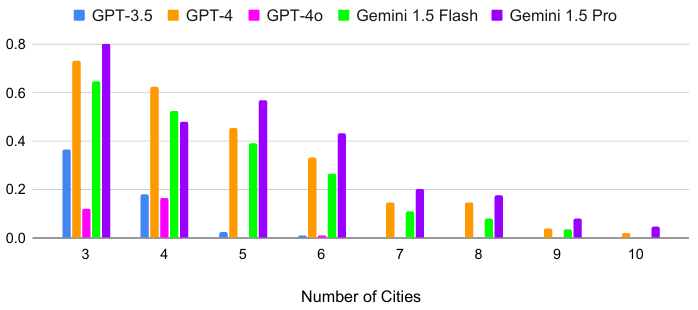
\includegraphics[width=0.7\textwidth]{images/image11.png}
\caption{เปรียบเทียบแนวโน้มประสิทธิภาพของ LLM เมื่อระดับความซับซ้อนและจำนวนเมืองในแผนการเดินทางเพิ่มขึ้น (Zheng et al., 2024)}
\end{figure}

ผลการศึกษาของ Zheng et al. (2024) ชี้ให้เห็นว่าเมื่อจำนวนเมืองและข้อจำกัดเพิ่มขึ้นจาก 2 เมืองเป็น 5 ถึง 10 เมือง อัตราความถูกต้องในการสร้างแผนงานของโมเดลภาษาชั้นนำอย่าง GPT-4o และ Gemini 1.5 Pro จะลดลงอย่างรุนแรงจนเหลือต่ำกว่าร้อยละ 5 ซึ่งสะท้อนถึงข้อจำกัดของโมเดลภาษาในการประมวลผลข้อจำกัดเชิงตัวเลข เวลา และตรรกะซับซ้อนด้วยตนเองเพียงอย่างเดียว

จากการสังเคราะห์ผลงานวิจัยของ Xie et al. (2024) และ Zheng et al. (2024) โครงงาน Dino จึงได้นำแนวคิดการประเมินข้อจำกัด 3 ระดับ ได้แก่ ข้อจำกัดเชิงสภาพแวดล้อม ข้อจำกัดเชิงสามัญสำนึก และข้อจำกัดตามเงื่อนไขผู้ใช้ มาประยุกต์ใช้เป็นเกณฑ์ประเมินเชิงปริมาณในส่วนการทดสอบประสิทธิภาพของระบบวางแผนการเดินทาง ควบคู่กับการนำแนวคิดการประเมินแบบ LLM-as-a-Judge และกลไก RAG มาใช้วัดผลความถูกต้องเชิงบริบทของระบบตอบโต้ เพื่อป้องกันการหลอนข้อมูล และส่งมอบแผนการท่องเที่ยวจังหวัดขอนแก่นที่มีความถูกต้อง สมเหตุสมผล และตรงตามความต้องการของผู้ใช้งานอย่างมีประสิทธิภาพ

\subsection{สรุปผลการเปรียบเทียบงานวิจัยที่เกี่ยวข้อง}

จากการทบทวนวรรณกรรมข้างต้น สามารถสรุปผลการเปรียบเทียบได้ดังตารางที่ \ref{tab:compare_research}

\begin{table}[H]
\centering
\caption{เปรียบเทียบงานวิจัยที่เกี่ยวข้อง}
\label{tab:compare_research}
\begin{tabular}{|p{3.4cm}|c|c|c|c|}
\hline
\textbf{งานวิจัย} & \textbf{RAG / LLM} & \textbf{Recomm.} & \textbf{Chatbot} & \textbf{Trip Planning} \\
\hline
\textcite{banerjee2025} & \cmark & \cmark & -- & -- \\ \hline
\textcite{jyothi2025} & -- & \cmark & -- & \cmark \\ \hline
\textcite{goizha2023} & -- & -- & \cmark & -- \\ \hline
\textcite{deshmukh2025} & -- & \cmark & \cmark & \cmark \\ \hline
\textcite{shao2025} & \cmark & -- & -- & \cmark \\ \hline
\textcite{barua2024} & -- & -- & -- & \cmark \\
\hline
\textbf{โครงงานนี้ (Dino)} & \cmark & \cmark & \cmark & \cmark \\
\hline
\end{tabular}
\end{table}

จากการวิเคราะห์งานวิจัยทั้ง 11 ชิ้น พบว่าแนวโน้มหลักของการวิจัยด้าน AI ในการท่องเที่ยว มุ่งเน้นไปที่การสร้างประสบการณ์การท่องเที่ยวที่เป็นส่วนบุคคลมากขึ้น และการพัฒนาระบบสนับสนุนการตัดสินใจของผู้ใช้ อย่างไรก็ตาม เมื่อสังเคราะห์เนื้อหาของงานวิจัยพบว่า ช่องว่างองค์ความรู้ที่สำคัญยังคงอยู่ในประเด็น การบูรณาการข้อมูลหลายระบบเข้าด้วยกัน กล่าวคือแต่ละงานมักมุ่งเน้นความสามารถเพียงด้านใดด้านหนึ่ง (การแนะนำ, Chatbot, การวางแผนทริป, การประเมินผล หรือสถาปัตยกรรมระบบ) โดยยังไม่มีงานใดผสานทั้ง RAG-based Recommendation, Chatbot แบบเรียลไทม์, ระบบวางแผนทริป และกรอบการประเมินผลแบบ LLM-as-a-Judge เข้าไว้ในแพลตฟอร์มเดียวกัน นอกจากนี้ แม้ \textcite{xie2024} และ \textcite{zheng2024} จะได้สร้าง Benchmark ประเมินผลระดับสากลไว้แล้ว แต่กรอบการประเมินส่วนใหญ่ยังจำกัดอยู่ในข้อมูลระดับโลกหรือข้อมูลจำลอง ยังขาดการประยุกต์ใช้กับระบบท่องเที่ยวระดับพื้นที่ (Local Tourism) เช่น จังหวัดขอนแก่น ซึ่งเป็นช่องว่างที่โครงงาน Dino มุ่งเข้าไปแก้ไข นอกจากนี้ \textcite{sousa2024} และ \textcite{milton2023} ยังชี้ให้เห็นถึงความท้าทายด้าน ความเป็นส่วนตัวของข้อมูลและธรรมาภิบาล ซึ่งยังไม่ได้รับการแก้ไขอย่างสมบูรณ์ในงานวิจัยส่วนใหญ่

\subsection{เทคโนโลยีและเครื่องมือที่เกี่ยวข้อง}

\subsubsection{Frontend: React}

ใช้ React ในการพัฒนาส่วนติดต่อผู้ใช้ ทั้งฝั่งเว็บและฝั่งมือถือ (Web/Mobile) เพื่อสร้างส่วนติดต่อผู้ใช้แบบ component-based ที่นำกลับมาใช้ซ้ำได้และอัปเดตข้อมูลแบบเรียลไทม์

\subsubsection{Backend: Node.js (Express) และ Python (FastAPI)}

ระบบฝั่งเซิร์ฟเวอร์แบ่งเป็น 2 บริการอิสระต่อกัน (Independent Services) คือ Backend API พัฒนาด้วย Node.js ร่วมกับเฟรมเวิร์ก Express สำหรับให้บริการ RESTful API ทั่วไปของระบบ และ AI Service พัฒนาด้วย Python ร่วมกับเฟรมเวิร์ก FastAPI แยกต่างหากสำหรับส่วนที่เกี่ยวข้องกับปัญญาประดิษฐ์และ RAG Pipeline โดยทั้งสองบริการสื่อสารระหว่างกันผ่าน RESTful API เท่านั้น ยังไม่มี API Gateway หรือ Message Broker ในระยะต้นแบบนี้

\subsubsection{ฐานข้อมูล: PostgreSQL พร้อมส่วนขยาย pgvector}

ใช้ฐานข้อมูล PostgreSQL (ผ่านบริการ Supabase) ที่มีส่วนขยายสำหรับจัดเก็บและค้นคืนข้อมูลเชิงเวกเตอร์ (pgvector) เป็นแหล่งจัดเก็บข้อมูลแบบรวมศูนย์ ทั้งข้อมูลทั่วไปของระบบ (เช่น ข้อมูลสถานที่ ผู้ใช้ กิจกรรม) และ Embeddings ที่ใช้ในการสืบค้นข้อมูลของระบบ RAG ไว้ในฐานข้อมูลเดียวกัน โดยเวกเตอร์ฝังตัวสร้างขึ้นด้วยโมเดล paraphrase-multilingual-MiniLM-L12-v2 (384 มิติ) ผ่านไลบรารี sentence-transformers ซึ่งประมวลผลบนเครื่องคอมพิวเตอร์ในเครื่อง (Local Inference)

\subsubsection{AI \& Libraries: LLM ผ่าน OpenAI-compatible API}

ใช้โมเดลภาษาขนาดใหญ่ (LLM) gemini-2.5-flash ผ่านช่องทาง API ที่รองรับมาตรฐาน OpenAI-compatible ร่วมกับไลบรารีสำหรับสร้าง RAG Pipeline เพื่อสนับสนุนระบบแชตบอตและระบบวางแผนการเดินทาง

\subsubsection{API ภายนอก: Google Places API}

ใช้ Google Places API สำหรับดึงข้อมูลตั้งต้น (Data Seeding) ของสถานที่ท่องเที่ยว ร้านอาหาร และกิจกรรมในจังหวัดขอนแก่น